\documentclass[border=0pt]{standalone}

\usepackage{enumitem}

\usepackage[sc]{mathpazo}
\usepackage{tikz}
\linespread{1.05}

\newcommand\bluebullet{%
  \tikz[baseline=0ex]\fill[blue!75!black]
    (0,0)--(0.18,0.09)--(0,0.18)--cycle;}


\usepackage[table]{xcolor}
\definecolor{petrol}{RGB}{127,173,198}


\usepackage{tikz}
\usetikzlibrary{calc}


\usepackage{ragged2e}

\begin{document}
\small

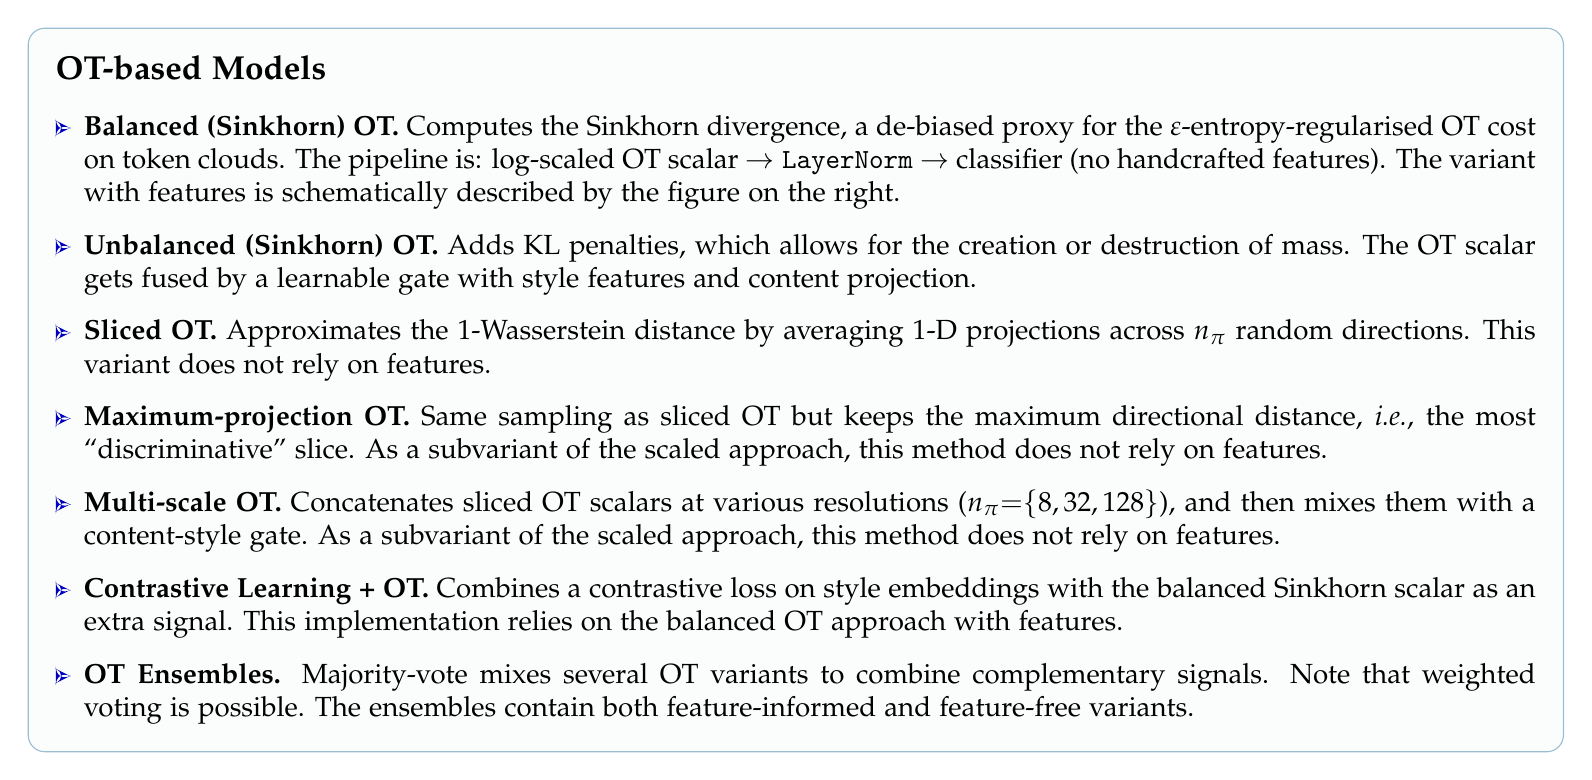
\begin{tikzpicture}
\node[
  draw=petrol!80,              
  fill=petrol!3,              
  rounded corners=6pt,
  minimum width=0.1\linewidth, 
  inner sep=10pt,               
  text width=1.55\linewidth, 
  font=\normalsize,
  align=justify                
] (cap) {%
  \noindent {\large\textbf{OT-based Models}}
\begin{itemize}[label=\bluebullet,left=0em,itemsep=3pt]
 \item \textbf{Balanced (Sinkhorn) OT.}  Computes the Sinkhorn divergence, a de-biased proxy for the $\varepsilon$-entropy-regularised OT cost on token clouds. The pipeline is: log-scaled OT scalar $\rightarrow$ \texttt{LayerNorm} $\rightarrow$ classifier (no handcrafted features). The variant with features is schematically described by the figure on the right.
  \item \textbf{Unbalanced (Sinkhorn) OT.}  Adds KL penalties, which allows for the creation or destruction of mass. The OT scalar gets fused by a learnable gate with style features and content projection.
  \item \textbf{Sliced OT.}  Approximates the 1-Wasserstein distance by averaging 1-D projections across $n_\pi$ random directions. This variant does not rely on features.
  \item \textbf{Maximum-projection OT.}  Same sampling as sliced OT but keeps the maximum directional distance, \textit{i.e.}, the most ``discriminative'' slice. As a subvariant of the scaled approach, this method does not rely on features.
  \item \textbf{Multi-scale OT.}  Concatenates sliced OT scalars at various resolutions ($n_\pi{=}\{8,32,128\}$), and then mixes them with a content-style gate. As a subvariant of the scaled approach, this method does not rely on features.
  \item \textbf{Contrastive Learning + OT.} Combines a contrastive loss on style embeddings with the balanced Sinkhorn scalar as an extra signal. This implementation relies on the balanced OT approach with features.
  \item \textbf{OT Ensembles.}  Majority-vote mixes several OT variants to combine complementary signals. Note that weighted voting is possible. The ensembles contain both feature-informed and feature-free variants.
\end{itemize}
  };
\end{tikzpicture}

\end{document}